\section{Model}

\subsection{Implementation of the model in linear programming}
\label{sec:model}
In order to compute the winning distribution law of the RCVS, one can implement a linear formulation of the model.
The linear formulation is based on the following variables:
\begin{itemize}
  \item $\pi$ the voting matrix where $\pi_{i,j}$ represents the results of a duel between the $i$-th and $j$-th candidates.
  The elements of the matrix are computed following this rule : for each voter, if the $i$-th canditate is ranked higher than the $j$-th candidate the element $\pi_{i,j}$ is incremented
  and the element $\pi_{j,i}$ is decremented.
  \item $p$ the probability vector where $p_i$ represents the probability that the $i$-th candidate wins.
  \item $e$ the vector of ones.
\end{itemize}

The linear formulation of the model is the following:
\begin{align*}
  &\max_{p} 1\\
  \text{s.t. } &p^T e = 1\\
  &p \geq 0\\
  &p^T \pi \geq 0  
\end{align*}

This formulation was implemented in the file \verb|q1_model.jl| using the \verb|JuMP| and \verb|Gurobi| packages.

\subsection{Application of the RCVS to an example}
One can apply the Condorcet winning system to the following example where edges goes from loser to winner with relatives voting preferences :

\begin{figure}[!h]
  \centering
  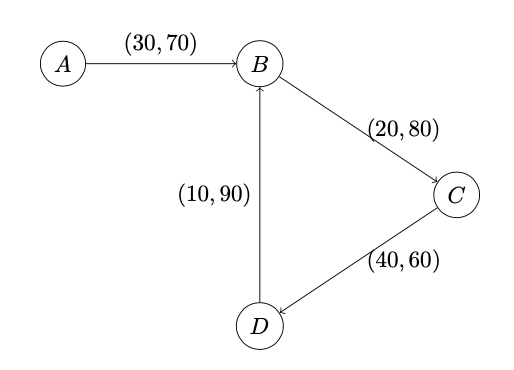
\includegraphics[width=0.5\textwidth]{figs/graph.png}
  \caption{Example of voting graph}
  \label{fig:q1_example}
\end{figure}

In this example, there will no be any Condorcet winner because the graph is not a directed acyclic graph, indeed there is a cycle between the candidates $B$, $C$ and $D$.
The RCVS is then needed to solve this problem. We simply need to compute the $\pi$ matrix respecting the graph represented in figure \ref{fig:q1_example} following the rule described in section \ref{sec:model}:

$$\pi = \begin{pmatrix}
  0 & -40 & 0 & 0\\
  40 & 0 & -60 & 80\\
  0 & 60 & 0 & -20\\
  0 & -80 & 20 & 0
\end{pmatrix}$$
\newpage
When launching the \verb|q1_model.jl| file with this matrix as input, we obtain the following lottery for the RCVS :

\begin{table}[!h]
  \centering
  \begin{tabular}{|c|c|c|c|c|}
  \hline
  Candidate   & $A$   & $B$     & $C$   & $D$     \\ \hline
  Probability & $0.0$ & $0.125$ & $0.5$ & $0.375$ \\ \hline
  \end{tabular}
  \caption{Lottery probabilities for each candidate}
  \label{tab:q1_prob}
\end{table}

\subsection{Discussion of the dual variables and optimal dual basis}
By using the following objective function : 
$$\max_p 1$$
We ensure that the algorithm will stop at the first iteration it finds a feasible basis and that the five dual variables are equal to $0$. We can easily check this affirmation by using the function \verb|solution_summary| and as expected the dual variables values are the following :

\begin{table}[!h]
\centering
\begin{tabular}{|c|c|c|c|c|c|}
\hline
Variable & $c_1[1]$ & $c_1[2]$ & $c_1[3]$ & $c_1[4]$ & $c_2$ \\ \hline
Value    & 0        & 0        & 0        & 0        & 0     \\ \hline
\end{tabular}
\caption{Dual variables values}
\label{tab:dual_q1_values}
\end{table}

This insures that the optimal was found because the dual variables represent the costs necessary to beat a candidate in a election and the optimal solution beats all the candidates. More formally, as our objective function is a constant, the relative costs $c^T$ are always equal to $0$ in each election. 

\subsection{Solution of the linear in a linear system}
By considering the following variables : 

$$A = \begin{pmatrix}0 & -40 & 0 & 0\\40 & 0 & -60 & 80\\0 & 60 & 0 & -20\\0 & -80 & 20 & 0\\1 & 1 & 1 & 1\end{pmatrix} 
\text{ , } 
x = \begin{pmatrix}p_1\\p_2\\p_3\\p_4\end{pmatrix} 
\text{ , } 
b = \begin{pmatrix}0\\0\\0\\0\\1\end{pmatrix}
\text{ , } 
d = \begin{pmatrix}d_1\\d_2\\d_3\\d_4\\d_5\end{pmatrix}
\text{ , }
c = \begin{pmatrix}1\\1\\1\\1\end{pmatrix}$$

We can create a system of 9 equations with 9 variables by considering that the 2 vectors of variables will be feasible for the primal and dual problems and optimal by considering : 

$$\begin{aligned}\begin{cases}
    \left(A^T_ix-b_i\right)d_i=0, &\forall i\\
    x_i\left(c_i-d^TA_i\right)=0, &\forall i
\end{cases}\end{aligned}$$

\subsection{\textit{Bonus} : Comparison of the RCVS with an alternative voting system}
One could compare the Randomized Condorcet Voting System with a much more simpler voting system as the two-round system used in a lot of countries to determine the winner of an election. This system is separated, as the name suggests, in two rounds :
\begin{itemize}
    \item In the first round, one could use his vote for every possible candidate on the list. The votes are then counted to determine the two candidates with the most votes.
    \item In the second round, all the voters can vote either for one or the other candidate previously selected in the first round. The winner of the election would be the one with the most votes.
\end{itemize}

Let there be an election between 3 candidates with 100 voters, the preferences of voters are summarized in the table below :

\begin{table}[!h]
\centering
\begin{tabular}{|c|c|}
\hline
Preference  & Voters \\ \hline
$A > B > C$ & 30     \\ \hline
$A > C > B$ & 5      \\ \hline
$B > A > C$ & 5      \\ \hline
$B > C > A$ & 25     \\ \hline
$C > A > B$ & 25     \\ \hline
$C > B > A$ & 10     \\ \hline
\end{tabular}
\caption{Preferences of voters}
\label{tab:preferences_1.5}
\end{table}

\begin{figure}[!h]
    \centering
    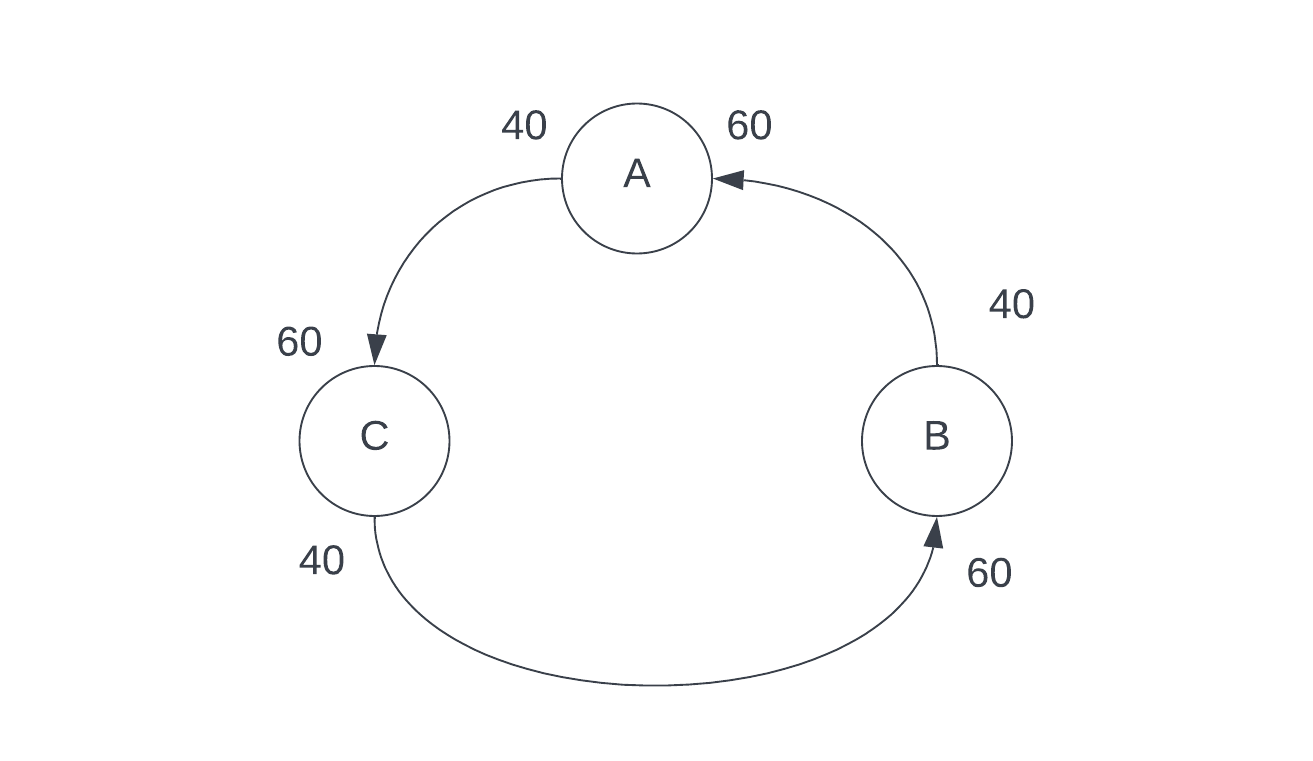
\includegraphics[width=.5\textwidth]{figs/graph_Q1_5.png}
    \caption{Duels graph}
    \label{fig:duel_graph_1.5}
\end{figure}

\paragraph{}
On one hand, if the system used was the two-round system, the two candidates selected in the first round would be $A$ and $C$ and if the preferences remained the same between rounds, the candidate $C$ would be elected with $60\%$ of the votes.
\paragraph{}
On the other hand, if the system used was the RCVS, we would obtain a Condorcet paradox (a cycle would appear in the duels graph). The resulting lottery values would be :

\begin{table}[!h]
\centering
\begin{tabular}{|c|c|}
\hline
Candidate & Probability   \\ \hline
$p(A)$    & $0.33$ \\ \hline
$p(B)$    & $0.33$ \\ \hline
$p(C)$    & $0.33$ \\ \hline
\end{tabular}
\caption{Winning lottery values}
\label{tab:prob_q1.5}
\end{table}